\documentclass{beamer}
\usepackage[utf8]{inputenc}
\usepackage{amsmath}
\usepackage{amssymb}
\usepackage{amsthm}
\usepackage{amscd}
\usepackage{amsfonts}
\usepackage{mathtools}
\usepackage{xcolor}
\usepackage{graphicx}
\usepackage{hyperref}
\usepackage{epigraph}
\usepackage[backend=biber, style=alphabetic, sorting=ynt]{biblatex}

\usetheme{Madrid}
\usecolortheme{default}
\setbeamertemplate{navigation symbols}{}
\setbeamertemplate{caption}[numbered]

% Commands from style.tex
\newtheorem{proposition}{Proposition}
\newtheorem{remark}{Remark}
\newtheorem{theorem}{Theorem}
\newtheorem{lemma}{Lemma}
\newtheorem{definition}{Definition}

\newcommand{\RR}[0]{\mathbb{R}}
\newcommand{\EE}[0]{\mathbb{E}}
\newcommand{\bx}[0]{{\bf x}}
\newcommand{\bv}[0]{{\bf v}}
\newcommand{\balpha}[0]{{\bf\alpha}}
\newcommand{\HH}{\mathcal{H}}
\newcommand{\heff}{\bar h^{\text{eff}}}

\title[A Mean Field Game Model For Educational Choices]{A Mean Field Game Model For Educational Choices}
\author{Felipe Antunes}
\institute{}
\date{\today}

\addbibresource{../sample.bib}

\begin{document}

\begin{frame}
\titlepage
\end{frame}

\begin{frame}{Outline}
\tableofcontents
\end{frame}

\section{Introduction}

\begin{frame}{Introduction to Mean Field Games}
\begin{quote}
\itshape ''[T]hey devote a very small fraction of the time to the consideration of any public object, most of it to the prosecution of their own objects. Meanwhile each fancies that no harm will come of his neglect, that it is the business of someone else to look after this or that for him; and so, by the same notion being entertained by all separately, the common cause imperceptibly decays''

\normalfont ---Thucydides - \textit{The history of the Peloponnesian War}
\end{quote}

\begin{itemize}
    \item A branch of game theory focusing on games with an infinite number of identical (symmetric) players
    \item Players are represented by their probability distribution over the state space
    \item Interaction between a representative player and the distribution
    \item Nash equilibria described by optimality conditions with a forward-backward structure
\end{itemize}
\end{frame}

\begin{frame}{Key Concepts in Mean Field Games}
\begin{itemize}
    \item Forward equation: Evolution of the distribution of players
    \item Backward equation: Optimization problem for the representative player
    \item Analytical approach: Fokker-Plank PDE with initial condition and Hamilton-Jacobi-Bellman PDE with terminal condition
    \item Probabilistic approach: Forward-Backward SDE with McKean-Vlasov interactions
\end{itemize}
\end{frame}

\begin{frame}{Economic Example - Introduction}
\begin{itemize}
    \item Example from economics to illustrate the mean field games methodology
    \item Mean field interactions arise naturally from the underlying economic theory
    \item Similar in nature to the educational model proposed
    \item Deterministic setting using Pontryagin's Maximum Principle
\end{itemize}
\end{frame}

\begin{frame}{Economic Example - Model}
\begin{itemize}
    \item $N$ agents with capital $k_0^i$ controlling consumption $c_t^i$
    \item Capital dynamics: $\dot k_t^i = \left( \left[r_t - \delta \right] k_t^i - c_t^i \right)\, dt$
    \item Aggregate production: $Y_t = F(\bar k_t)$, where $\bar k_t = \frac{1}{N} \sum_{i = 1}^N k_t^i$
    \item Interest rate determined by marginal effect of capital: $r_t = \partial_K Y = C \bar k_t$
    \item Optimization problem: 
    \begin{equation}
        \max_{c^i } \int_0^T u(c^i_s) ds + \psi(k^i_T)
    \end{equation}
\end{itemize}
\end{frame}

\begin{frame}{Economic Example - Mean Field Approximation}
\begin{itemize}
    \item Replace $N$ players with a probability measure flow $\mu_t$
    \item Nash equilibrium: $\mu_t^*$ such that $\mu_t^* = O(\mu_t^*)$
    \item Pattern of analysis:
    \begin{enumerate}
        \item Find optimal control for a representative player given $\mu_t$
        \item Derive the induced flow $O(\mu_t)$
        \item Find fixed point $\mu_t^* = O(\mu_t^*)$
    \end{enumerate}
    \item Representative agent's optimization problem:
    \begin{equation}
        \max_{c} \int_0^T \log(c_s) ds -\frac{1}{2}{(k_T)}^2
    \end{equation}
\end{itemize}
\end{frame}

\begin{frame}{Economic Example - MFG System}
\begin{itemize}
    \item Forward-backward system of ODEs:
    \begin{equation}
        \begin{cases}
             d k_t = \left(\left[ C {\hat k_t} - \delta \right] k_t - \frac{1}{p_t} \right)\, dt,\\
             d p_t = - \left( \left[C{\hat k_t} - \delta \right] p_t \right) \, dt, \\
             k_0 \sim \mu_0,\, p_T =  - k_T.         
        \end{cases}
    \end{equation}
    \item PDE system:
    \begin{equation}
        \begin{cases}
            \partial_t V +  \left(C {\bar k_t(\rho) - \delta}\right)k\partial_k V - 1  - \log(\partial_k V) = 0 \\
            \partial_t \rho - \partial_k \left( \left[ \left(C {\bar k_t}(\rho) - \delta\right) k - {(\partial_k V)}^{-1} \right]\rho \right) = 0
        \end{cases}
    \end{equation}
\end{itemize}
\end{frame}

\section{Theoretical Review}

\begin{frame}{Theoretical Review - Overview}
\begin{itemize}
    \item Mean field games are a framework for approximating Nash equilibria in large player games
    \item Two equivalent formulations:
    \begin{itemize}
        \item System of coupled partial differential equations
        \item System of forward-backward stochastic differential equations
    \end{itemize}
    \item Key theoretical components:
    \begin{itemize}
        \item Stochastic optimal control
        \item Wasserstein spaces
        \item Convergence of $N$-player game to MFG system
    \end{itemize}
\end{itemize}
\end{frame}

\begin{frame}{Stochastic Optimal Control - Key Concepts}
\begin{itemize}
    \item Controlled stochastic differential equation:
    \begin{equation}
        d X_s = b(X_s, \alpha_s)ds + \sigma(X_s, \alpha_s) d W_s
    \end{equation}
    \item Objective function:
    \begin{equation}
        J(t, x, \alpha) = \mathbb{E}\left[ \int_t^T f(s, X_s^{t,x}, \alpha_s) ds + g(X^{t,x}_T) \right]
    \end{equation}
    \item Value function:
    \begin{equation}
        v(t,x) = \sup_{\alpha \in \mathcal{A}(t,x)} J(t,x,\alpha)
    \end{equation}
\end{itemize}
\end{frame}

\begin{frame}{Dynamic Programming Principle}
\begin{theorem}[Dynamic Programming Principle]
    The value function $v$ satisfies:
    \begin{gather} 
        v(t,x) = \sup_{\alpha \in \mathcal{A}(t,x)}
        \sup_{\theta \in \mathcal{T}_{t,T}}
        \mathbb{E}\left[ \int_t^\theta f(s, X_s^{t,x}, \alpha_s) ds + v(\theta, X^{t,x}_\theta) \right]
    \end{gather}
    where $\mathcal{T}_{t, T}$ is the set of stopping times valued in $[t,T]$.
\end{theorem}

\begin{itemize}
    \item Leads to the Hamilton-Jacobi-Bellman (HJB) equation:
    \begin{equation}
        -\frac{\partial v}{\partial t} - H(t,x,\partial_x v, \partial_{xx} v) = 0
    \end{equation}
    \item Terminal condition: $v(T,x) = g(x)$
\end{itemize}
\end{frame}

\begin{frame}{Viscosity Solutions}
\begin{definition}[Second Order Viscosity Solutions]
    \begin{itemize}
        \item A function $u$ is a viscosity subsolution if
        $F(x_0, u(x_0), D \phi(x_0), D^2 \phi(x_0)) \leq 0$
        for all test functions $\phi$ at maximum points of $u - \phi$
        
        \item A function $u$ is a viscosity supersolution if
        $F(x_0, u(x_0), D\phi(x_0), D^2 \phi(x_0)) \geq 0$
        for all test functions $\phi$ at minimum points of $u - \phi$
        
        \item A function $u$ is a viscosity solution if it is both a subsolution and a supersolution
    \end{itemize}
\end{definition}

\begin{itemize}
    \item Essential for dealing with non-smooth value functions
    \item Ensures uniqueness of solutions through comparison principles
\end{itemize}
\end{frame}

\section{Proposed Model}

\begin{frame}{Model Introduction}
\begin{itemize}
    \item Game theoretical model for time allocation between work and education
    \item Based on Lucas's human capital growth model and Aiyagari's growth model
    \item Interactions mediated through interest rate and wage rate
    \item Motivated by high rate of school evasion in Brazil due to necessity of working
    \begin{itemize}
        \item 45\% of people out of school (15-29 years old) cite work needs as reason for not pursuing education
    \end{itemize}
    \item Expected outcomes:
    \begin{itemize}
        \item Qualitative properties of population behavior
        \item Numerical solutions of the mean field limit
        \item Modeling public policies to promote education
    \end{itemize}
\end{itemize}
\end{frame}

\begin{frame}{Model Description}
\begin{itemize}
    \item $N$ agents with wealth $A_t$ and skill level $H_t$
    \item Controls: consumption $c_t$ and proportion of time dedicated to working $u_t$
    \item Proportion $1-u_t$ used for improving skill level
    \item Optimization problem:
    \begin{equation}
    \begin{cases}
        \sup\limits_{(u,c) \in \mathcal{U} \times \mathcal{C}}\mathbb{E} [ \int_0^T f_c(c^i_s) + f_u(u^i_s) ds + Q(A^i_T) ]\\
        d A^i_t = \left[ (\bar r_t - \delta) A^i_t + \bar w_t H^i_t u^i_t - c^i_t  \right] dt + \sigma_a A^i_t d W^{a,i}_t\\
        d H^i_t = (H^i_t)^\xi g(1 - u^i_t) dt + \sigma_h H^i_t d W^{h,i}_t
    \end{cases}
    \end{equation}
\end{itemize}
\end{frame}

\begin{frame}{Wealth and Skill Dynamics}
\begin{itemize}
    \item Wealth dynamics:
    \begin{itemize}
        \item Interest returns: $(\bar r_t - \delta) A_t$
        \item Wages: $\bar w_t H_t u_t$ (proportional to time and skill)
        \item Consumption: $-c_t$
        \item Noise term: $\sigma_a A_t d W^a_t$
    \end{itemize}
    \item Skill dynamics:
    \begin{itemize}
        \item Skill improvement: $H^\xi_t g(1 - u_t) dt$
        \item Parameter $\xi$ captures impact of current skill on effectiveness
        \item Noise term: $\sigma_h H_t dW^h_t$
    \end{itemize}
\end{itemize}
\end{frame}

\begin{frame}{Mean Field Interactions}
\begin{itemize}
    \item Interaction mediated through $\bar r_t$ and $\bar w_t$
    \item Cobb-Douglas production function $F$ depending on:
    \begin{itemize}
        \item Average wealth $\bar a_t$
        \item Effective supply of skilled labor $\heff_t$
    \end{itemize}
    \item Agents distributed with measure $\mu^N_t \in \mathcal{P}(\Omega)$
    \item At economic equilibrium:
    \begin{align}
        \bar r(\mu^N_t) &= \partial_a F(\bar a(\mu^N_t), \heff(\mu^N_t))\\
        \bar w(\mu^N_t) &= \partial_h F(\bar a(\mu^N_t), \heff(\mu^N_t))
    \end{align}
\end{itemize}
\end{frame}

\begin{frame}{MFG Analytic System}
For Nash equilibria as $N \to \infty$:
\begin{equation}
    \begin{cases}
        \partial_t V + (\bar r  - \delta) a \partial_a V + \HH_u(h, \partial_a V, \partial_h V)  + \HH_c(\partial_a V) \\
        \quad\quad + \frac{1}{2} \sigma_a^2 a^2 \partial_{aa} V + \frac{1}{2} \sigma^2_h h^2 \partial_{hh} V = 0,\\
        \partial_t \mu + \partial_a \left( \left[ (\bar r - \delta) a + \partial_p \HH_u(h, \partial_a V, \partial_h V) + \partial_p \HH_c(\partial_a V) \right] \mu \right) \\
        \quad\quad + \partial_h \left( \partial_q \HH_u(h, \partial_a V, \partial_h V)\, \mu\right) \\
        \quad\quad - \frac{1}{2} \sigma_a^2 \partial_{aa} (a^2\mu) - \frac{1}{2} \sigma^2_h \partial_{hh} (h^2\mu) = 0,\\
        \mu(0,a,h) = \mu_0,\quad V(T,a,h) = Q(a)
    \end{cases}
\end{equation}

where $\HH_u$ and $\HH_c$ are Hamiltonian functions for the optimization problems
\end{frame}

\begin{frame}{MFG FBSDE System}
Alternative formulation with Forward-Backward SDEs:
\begin{equation}
    \begin{cases}
        d A_t = \left[ (\bar r_t - \delta) A_t + \bar w_t H_t {\hat u}_t - {\hat c}_t  \right] dt + \sigma_a A_t d W^a_t,\\
        d H_t = H^\xi_t g(1 - {\hat u}_t) dt + \sigma_h H_t d W^h_t,\\
        d P_t = -\left[ (\bar r_t - \delta) P_t + \sigma_a Z^p_t \right]dt + Z^p_t d W^a_t,\\
        d Q_t = - \left[ \xi H_t^{\xi - 1} g(1 - {\hat u}_t ) Q_t + {\bar w} {\hat u}_t P_t + \sigma_h Z^q_t \right] dt + Z^q_t d W^h_t,\\
        \mathcal{L}(A_0, H_0) = \mu_0, \, P_T = \partial_a Q(A_T), Q_T = 0
    \end{cases}
\end{equation}

With $\hat u_t \coloneqq \hat u(H_t,P_t,Q_t)$ and $\hat c_t \coloneqq \hat c(P_t)$
\end{frame}

\begin{frame}{Numerical Illustration}
\begin{itemize}
    \item $N$-player deterministic version simulated through adapted shooting algorithm
    \item Simplified model:
    \begin{itemize}
        \item $g(1- u) = (1 - u)$, $\xi = 0$, $\delta = 0.05$, $k = 0.5$
        \item $f_c(c) = \log(c)$, $f_u(u) = -\frac{\alpha}{2} u^2$, $Q(a) = a$
    \end{itemize}
    \item Two scenarios: $\alpha = 0.5$ vs $\alpha = 2$ (lower vs higher preference for education)
\end{itemize}

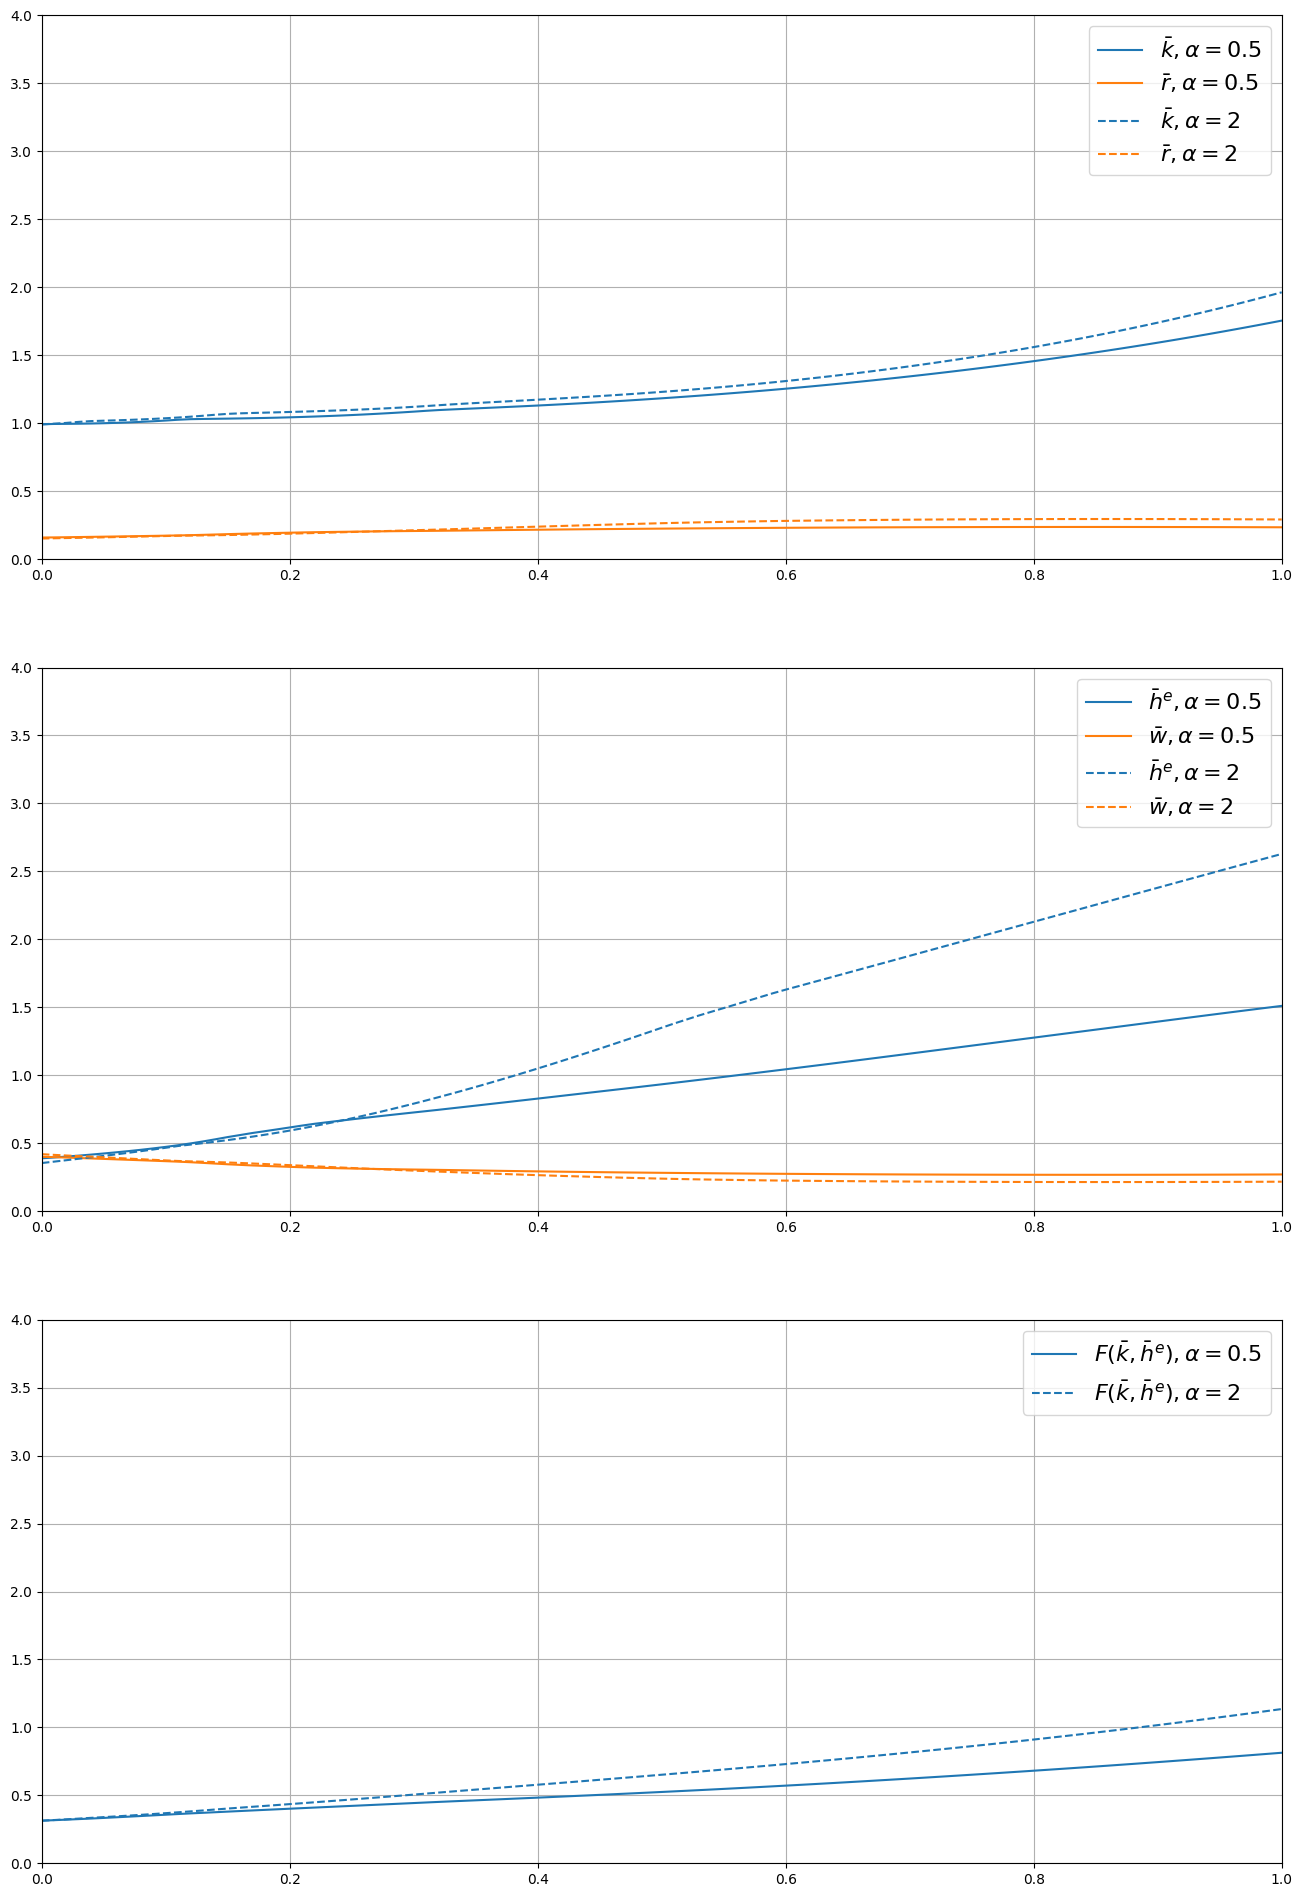
\includegraphics[width=0.85\textwidth]{../qualificacao/model_proposal/simulations/simulations_mfg.png}
\end{frame}

\begin{frame}{Simulation Results}
\begin{itemize}
    \item Increased preference for education leads to:
    \begin{itemize}
        \item Increased average wealth
        \item Higher interest rates
        \item Higher aggregate production
        \item Effective supply of skilled labor:
        \begin{itemize}
            \item Decrease in the short term
            \item Increase in the long term
        \end{itemize}
        \item Decreased wages per skill per time
    \end{itemize}
\end{itemize}
\end{frame}

\section{Conclusion}

\begin{frame}{Conclusion and Future Work}
\begin{itemize}
    \item Reviewed mean field game theory
    \item Proposed a model of effects of education preferences on the economy
    \item Next steps:
    \begin{itemize}
        \item Simulate full model using finite difference methods and machine learning
        \item Derive analytical results for the model
        \item Propose modifications to the baseline model
        \item Consider principal-agent mean field control problem:
        \begin{itemize}
            \item Decision maker optimizing public policy
            \item Associated utility over population distribution state
        \end{itemize}
    \end{itemize}
\end{itemize}
\end{frame}

\begin{frame}{Summary}
\begin{itemize}
    \item Mean Field Games provide a powerful framework for studying strategic interactions in large populations
    \item Educational choice model:
    \begin{itemize}
        \item Captures trade-off between work and education
        \item Shows how individual preferences affect aggregate outcomes
        \item Demonstrates the economic benefits of education
    \end{itemize}
    \item Applications:
    \begin{itemize}
        \item Educational policy design
        \item Understanding wealth and skill distribution dynamics
        \item Predicting economic impacts of educational incentives
    \end{itemize}
\end{itemize}
\end{frame}

\begin{frame}{References}
\printbibliography
\end{frame}

\end{document}